%%%%%%%%%%%%  Generated using docx2latex.pythonanywhere.com  %%%%%%%%%%%%%%


\documentclass[a4paper,12pt]{report}

% Other options in place of 'report' are 1)article 2)book 3)letter
% Other options in place of 'a4paper' are 1)a5paper 2)b5paper 3)letterpaper 4)legalpaper 5)executivepaper


 %%%%%%%%%%%%  Include Packages  %%%%%%%%%%%%%%


\usepackage{amsmath}
\usepackage{latexsym}
\usepackage{amsfonts}
\usepackage{amssymb}
\usepackage{graphicx}
\usepackage{txfonts}
\usepackage{wasysym}
\usepackage{enumitem}
\usepackage{adjustbox}
\usepackage{ragged2e}
\usepackage{tabularx}
\usepackage{changepage}
\usepackage{setspace}
\usepackage{hhline}
\usepackage{multicol}
\usepackage{float}
\usepackage{multirow}
\usepackage{makecell}
\usepackage{fancyhdr}
\usepackage[toc,page]{appendix}
\usepackage[utf8]{inputenc}
\usepackage[T1]{fontenc}
\usepackage{hyperref}


 %%%%%%%%%%%%  Define Colors For Hyperlinks  %%%%%%%%%%%%%%


\hypersetup{
colorlinks=true,
linkcolor=blue,
filecolor=magenta,
urlcolor=cyan,
}
\urlstyle{same}


 %%%%%%%%%%%%  Set Depths for Sections  %%%%%%%%%%%%%%

% 1) Section
% 1.1) SubSection
% 1.1.1) SubSubSection
% 1.1.1.1) Paragraph
% 1.1.1.1.1) Subparagraph


\setcounter{tocdepth}{5}
\setcounter{secnumdepth}{5}


 %%%%%%%%%%%%  Set Page Margins  %%%%%%%%%%%%%%


\usepackage[a4paper,bindingoffset=0.2in,headsep=0.5cm,left=1.25in,right=1.25in,bottom=2cm,top=2cm,headheight=2cm]{geometry}
\everymath{\displaystyle}


 %%%%%%%%%%%%  Set Depths for Nested Lists created by \begin{enumerate}  %%%%%%%%%%%%%%


\setlistdepth{9}
\newlist{myEnumerate}{enumerate}{9}
	\setlist[myEnumerate,1]{label=\arabic*)}
	\setlist[myEnumerate,2]{label=\alph*)}
	\setlist[myEnumerate,3]{label=(\roman*)}
	\setlist[myEnumerate,4]{label=(\arabic*)}
	\setlist[myEnumerate,5]{label=(\Alph*)}
	\setlist[myEnumerate,6]{label=(\Roman*)}
	\setlist[myEnumerate,7]{label=\arabic*}
	\setlist[myEnumerate,8]{label=\alph*}
	\setlist[myEnumerate,9]{label=\roman*}

\renewlist{itemize}{itemize}{9}
	\setlist[itemize]{label=$\cdot$}
	\setlist[itemize,1]{label=\textbullet}
	\setlist[itemize,2]{label=$\circ$}
	\setlist[itemize,3]{label=$\ast$}
	\setlist[itemize,4]{label=$\dagger$}
	\setlist[itemize,5]{label=$\triangleright$}
	\setlist[itemize,6]{label=$\bigstar$}
	\setlist[itemize,7]{label=$\blacklozenge$}
	\setlist[itemize,8]{label=$\prime$}



 %%%%%%%%%%%%  Header here  %%%%%%%%%%%%%%


\pagestyle{fancy}
\fancyhf{}


 %%%%%%%%%%%%  Footer here  %%%%%%%%%%%%%%




 %%%%%%%%%%%%  Print Page Numbers  %%%%%%%%%%%%%%


\rfoot{\thepage}


 %%%%%%%%%%%%  This sets linespacing (verticle gap between Lines) Default=1 %%%%%%%%%%%%%%


\setstretch{1.15}


 %%%%%%%%%%%%  Document Code starts here %%%%%%%%%%%%%%


\title{Spatial IIR – math development}
\begin{document}
\maketitle
\sloppy 
 \par
\noindent 
\section*{Abstract}
 \par
\noindent 
\section*{Signal model}
 \par
\noindent 
\begin{center}

 %%%%%%%%%%%%  Figure/Image No:1 here %%%%%%%%%%%%%%


\begin{figure}[H]
\begin{center}
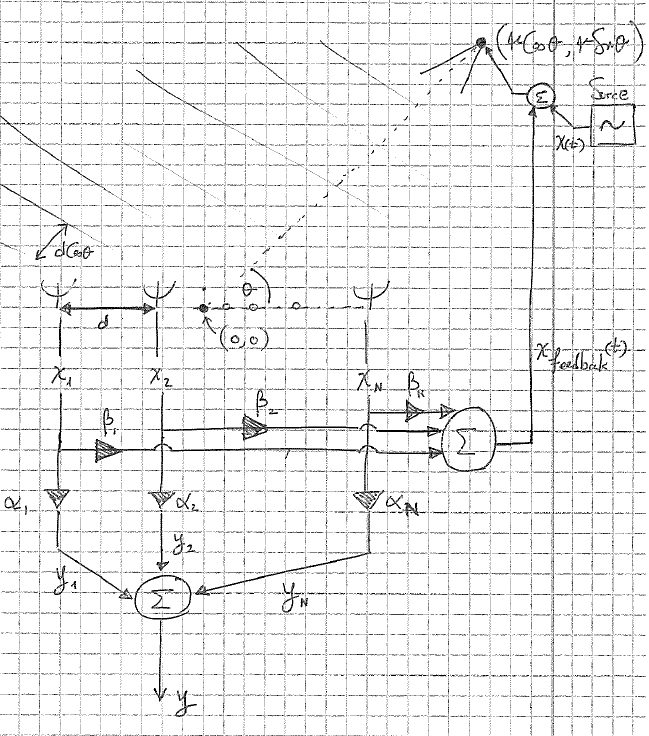
\includegraphics[width=4.57in,height=5.18in]{./Media/image1.png}
\end{center}
\end{figure}


 %%%%%%%%%%%%  Figure/Image No:1 Ends Here %%%%%%%%%%%%%%


\end{center}\vspace{12pt}
\vspace{12pt}
\noindent 
$$  \tau_{pd}=\frac{r}{c} $$
 \par
\noindent 
$  \tau \left(  \theta  \right) =\frac{dcos \left(  \theta  \right) }{c} $
 \par
\noindent 
$ x_{n} \left( t \right) =x \left( t- \left( n-1 \right)  \tau \left(  \theta  \right)  \right) + \sum _{m=1}^{N} \beta _{m}x_{m} \left( t- \tau_{pd}- \left( m-1 \right)  \tau \left(  \theta  \right)  \right)  $
 \par
\noindent 

 \par
\noindent 
Defining $ X \left(  \omega  \right) = \left[  \right]  $
 , \par
\noindent 
$ X \left(  \omega  \right) = \left[  \right] ~X \left(  \omega  \right) + \beta X \left(  \omega  \right)  \triangleq d \left(  \theta  \right) X \left(  \omega  \right) + \beta X \left(  \omega  \right)  $
 \par
\noindent 
$ X \left(  \omega  \right) = \left( I_{NxN}- \beta  \right) ^{-1}d \left(  \theta  \right) X \left(  \omega  \right)  $
 \par
\noindent 
\begin{center}$ Y \left(  \omega  \right) = \sum _{n=1}^{N} \alpha _{n}X \left(  \omega  \right) = \alpha ^{T} \left( I_{NxN}- \beta  \left(  \theta  \right)  \right) ^{-1}d \left(  \theta  \right) X \left(  \omega  \right)  $
,\end{center} \par
\noindent 
where \par
\noindent 
$  \beta =e^{-j \omega  \tau_{pd}} \left[  \right]  $
 \par
\vspace{12pt}
\noindent 
According to [1], if $ G $
 and $ H $
 are square matrices of same dimensions, where $ G $
 is invertible and $ H $
 is of rank 1, the inverse of their sum is \vspace{\baselineskip}
$  \left( G+H \right) ^{-1}=G^{-1}-\frac{1}{1+g}G^{-1}HG^{-1} $
where$ ~g=tr \left( HG^{-1} \right)  $
.\vspace{\baselineskip}
It can be easily seen that$ ~ \beta  $
 is of rank 1, and when setting $ G $
 as the identity matrix $ I $
 it follows that\vspace{\baselineskip}
$  \left( I+ \left( - \beta  \right)  \right) ^{-1}=I-\frac{1}{1+g} \left( - \beta  \right) g=tr \left( - \beta  \right) =e^{-j \omega  \tau_{pd}} \sum _{n=1}^{N} \left( - \beta _{n} \right) e^{j \omega  \left( n-1 \right)  \tau \left(  \theta  \right) } $
 \par
\noindent 
$  \Rightarrow  \left( I+ \beta  \right) ^{-1}=\frac{ \left( 1+e^{-j \omega  \tau_{pd}} \sum _{n=1}^{N} \left( - \beta _{n} \right) e^{j \omega  \left( n-1 \right)  \tau \left(  \theta  \right) } \right) I+ \beta }{1+e^{-j \omega  \tau_{pd}} \sum _{n=1}^{N} \left( - \beta _{n} \right) e^{j \omega  \left( n-1 \right)  \tau \left(  \theta  \right) }} \Rightarrow ~Y \left(  \omega  \right) = \sum _{n=1}^{N} \alpha _{n}X \left(  \omega  \right) =\frac{ \alpha ^{T} \left(  \left( 1-e^{-j \omega  \tau_{pd}} \sum _{n=1}^{N} \beta _{n}e^{j \omega  \left( n-1 \right)  \tau \left(  \theta  \right) } \right) I+ \beta  \right) d \left(  \theta  \right) }{1-e^{-j \omega  \tau_{pd}} \sum _{n=1}^{N} \beta _{n}e^{j \omega  \left( n-1 \right)  \tau \left(  \theta  \right) }}X \left(  \omega  \right)  $
And now, one can easily notice that the transfer function of the system is:\vspace{\baselineskip}
$ H \left(  \alpha , \beta , \omega , \theta  \right) =\frac{ \alpha ^{T} \left(  \left( 1-e^{-j \omega  \tau_{pd}} \sum _{n=1}^{N} \beta _{n}e^{j \omega  \left( n-1 \right)  \tau \left(  \theta  \right) } \right) I+ \beta  \right) d \left(  \theta  \right) }{1-e^{-j \omega  \tau_{pd}} \sum _{n=1}^{N} \beta _{n}e^{j \omega  \left( n-1 \right)  \tau \left(  \theta  \right) }} $
 \par
\noindent 


 %%%%%%%%%%%%  Start New Page here %%%%%%%%%%%%%%


\newpage

\vspace{14pt}
\noindent 
\section*{Design flow}
 \par
\noindent 
The coefficients determination flow will be as follows:  \par
\noindent 
\begin{itemize}
\item For each $  \omega  $
 \par
\noindent 
\begin{itemize}
\item Determine the wanted spatial IIR filter coefficients of order $ N-1 $
 which will generate a spatial transfer function of$ ~H \left(  \theta  \right)  $
. \par
\noindent 
\item Adjust $  \alpha  \left(  \omega  \right)  $
 and $  \beta  \left(  \omega  \right)  $
 to fit the wanted coefficients \par
\noindent 
\end{itemize}
\item  Design for each sensor $  \left( n \right)  $
 two digital filters, $  \alpha _{n} \left(  \omega  \right)  $
 and $  \beta _{n} \left(  \omega  \right)  $
 and the overall system will be a broad-band spatial IIR filter.\end{itemize}
 \par
\end{document}
